\documentclass[12pt]{article}
%\documentclass[border=0.1cm]{standalone}
\usepackage[super]{nth}
\usepackage{wasysym}
\usepackage{phonenumbers}
\usepackage{marvosym }
\usepackage{xcolor}
\usepackage{comment}
\usepackage{pdfpages}
\usepackage[paperwidth=8.5in,paperheight=11in,margin=0.5in]{geometry} 
\usepackage[UKenglish]{babel}
\usepackage[UKenglish]{isodate}% http://ctan.org/pkg/isodate
\usepackage[colorlinks=true,linkcolor=black,anchorcolor=black,citecolor=black,filecolor=black,menucolor=black,runcolor=black,urlcolor=black]{hyperref}
\usepackage[activate={true,nocompatibility},final,tracking=true,kerning=true,spacing=true,factor=1100,stretch=10,shrink=10]{microtype}
\frenchspacing
\usepackage[nodayofweek,level]{datetime}
\usepackage{calc,url}
\newcounter{qz}\setcounter{qz}{0}
\newcommand{\qz}{%\
\setcounter{qz}{\value{qz}+1}
\textbf{In-class  \theqz} \,}

\newcounter{hw}\setcounter{hw}{0}
\newcommand{\hw}{%\
\setcounter{hw}{\value{hw}+1}
\textbf{HW \thehw}}

\newcounter{ex}\setcounter{ex}{0}
\newcommand{\ex}{%\
\setcounter{ex}{\value{ex}+1}
Exam \theex}

\usepackage{fourier}
\usepackage[T1]{fontenc}

%\usepackage{tgschola} %to look retro
\newenvironment{mypar}[2]
  {\begin{list}{}%
    {\setlength\leftmargin{#1}
    \setlength\rightmargin{#2}}
    \item[]}
  {\end{list}}


\newcounter{wk}\setcounter{wk}{0}
\newcommand{\wk}{%\
\setcounter{wk}{\value{wk}+1}
\thewk \,\,}

\usepackage[nomessages]{fp}% http://ctan.org/pkg/fp


\usepackage{enumerate}
\usepackage{graphicx}

\usepackage{paralist}
\renewenvironment{description}[0]{\begin{compactdesc}}{\end{compactdesc}}

\newenvironment{alphalist}{
  \begin{enumerate}[(a)]
    \addtolength{\itemsep}{-0.5\itemsep}}
  {\end{enumerate}}
  \cleanlookdateon% Remove ordinal day reference
  \newcommand{\RomanNumeralCaps}[1]
      {\MakeUppercase{\romannumeral #1}}

\usepackage{xspace}
\makeatletter
\DeclareRobustCommand{\maybefakesc}[1]{%
  \ifnum\pdfstrcmp{\f@series}{\bfdefault}=\z@
    {\fontsize{\dimexpr0.8\dimexpr\f@size pt\relax}{0}\selectfont\uppercase{#1}}%
  \else
    \textsc{#1}%
  \fi
}
\newcommand\AM{\,\maybefakesc{am}\xspace}
\newcommand\PM{\,\maybefakesc{pm}\xspace}
\makeatother

 \newcommand{\coursename}{Calculus I with Analytic Geometry}
\newcommand{\coursenumber}{MATH 115}
\newcommand{\sectionnumber}{02}
\newcommand{\term}{Fall }
\newcommand{\room}{Discovery Hall, room  383}
\newcommand{\meetingtime}{This class meets Monday, Wednesday, and Friday  from 
	12:30\PM{}  --  1:10 \PM and Tuesday and Thursday from 12:30 \PM{} -- 1:10 \PM }
\newcommand{\officehours}{ Monday, Wednesday, and Friday 10:00\AM{} -- 11:00\AM,
    Tuesday and Thursday 9:30\AM -- 11:00\AM, and by appointment.}

    \newcommand{\finaldateandtime}{\printdate{15/12/\the\year},{} from 10:30\AM{} -- 12:30 \PM}
\begin{document}
\cleanlookdateon% Remove ordinal day reference
\shortdate
\printyearoff
\large
\begin{center}
    \textbf{\coursename}  \\
    {\coursenumber--\sectionnumber} \\
     {\term \the\year} \\
\end{center}

\vskip0.25in
\normalsize


\begin{center}
\begin{description}
    \item[Instructor:] Barton Willis, PhD, Professor of Mathematics
    \item[Office:]  Discovery Hall, Room 368
    \item[\phone:]   \phonenumber[country=US]{3088658868}
    \item[\Email:]    \href{mailto:willisb@unk.edu}{willisb@unk.edu}
    \item[Zoom:] 616 568 5706
    \item[Office Hours:] \officehours
  \end{description}
\end{center}



\subsubsection*{Important Dates}

\begin{mypar}{0.25in}{0.25in} 

      \textbf{First Online Homework due} \dotfill  \printdate{3/9/\the\year}  \\
       \textbf{Exam 1} \dotfill \printdate{23/9/\the\year}  \\
    \textbf{Exam 2} \dotfill  \printdate{4/11/\the\year} \\
    \textbf{Exam 3} \dotfill \printdate{2/12/\the\year} \\
     \textbf{Exam 4} \dotfill \printdate{12/12/\the\year},{} from 1:00 \PM{} -- 3:00 \PM \\
      \textbf{Final exam} \dotfill  \finaldateandtime
\end{mypar}


\subsubsection*{Class meeting times}

This class meets \meetingtime{} in \room.


\subsubsection*{Grading}

Your course grade will be based on weekly in class work, online homework, four midterm exams, and a comprehensive 
final exam; specifically:
\begin{mypar}{0.25in}{0.25in}
    \textbf{In class work}  \emph{15 ten point assignments}  \dotfill 150 (total) \\
     \textbf{Online homework} \emph{39 four point assignments }\dotfill 156 (total)\\
    \textbf{Mid-term Exams 1,2, and 3} \emph{100 points each} \dotfill 300 (total)\\
   \textbf{Exam 4} \emph{25 points} \dotfill 25 (total)\\ 
      \textbf{Comprehensive Final exam} \dotfill 150 (total)
\end{mypar}
Exam 4, worth 25 points covers the final two weeks of the course and it is given 
during final exam week. The comprehensive final exam, worth 150 points, is also 
given during final exam week. If we end the term with slightly fewer or more in class
assignments, your in class work score will be proportionally scaled to 150 points. The same 
scaling for online homework.

\FPeval{\points}{round(150+156+300+25+150,0)}

\FPeval{\F}{round(\points*0.6-1,0)}
\FPeval{\Dm}{round(\points*0.6,0)}
\FPeval{\D}{round(\points*0.633,0)}
\FPeval{\Dp}{round(\points*0.6667,0)}

\FPeval{\Cm}{round(\points*0.7,0)}
\FPeval{\C}{round(\points*0.733,0)}
\FPeval{\Cp}{round(\points*0.7667,0)}

\FPeval{\Bm}{round(\points*0.8,0)}
\FPeval{\B}{round(\points*0.833,0)}
\FPeval{\Bp}{round(\points*0.8667,0)}

\FPeval{\Am}{round(\points*0.9,0)}
\FPeval{\A}{round(\points*0.933,0)}
\FPeval{\Ap}{round(\points*0.98,0)}

The following table shows the \emph{minimum} number of points (out of \points) that
are required for each of the twelve letter grades D- through A+. For
example, a point total of \Bp\/  points will earn you a grade of B+,  and 
a point total of \Am\/ points will earn you a grade of A-. If you earn a point
total of \F\/  or less, you a failing course grade.
 
 \vspace{0.1in}
     \begin{minipage}{5.5in}
  \centering 
\begin{mypar}{0.25in}{0.25in}
    \begin{minipage}{2.5in}
        D-  \dotfill \Dm \\
        D \dotfill \D \\
        D+ \dotfill \Dp \\
        C- \dotfill \Cm  \\
        C \dotfill \C \\
        C+ \dotfill \Cp 
        \end{minipage}
    \phantom{xxx}
    \begin{minipage}{2.5in}
        B- \dotfill \Bm \\
        B \dotfill  \B \\
        B+ \dotfill  \Bp\\
        A- \dotfill  \Am \\
        A \dotfill  \A \\
        A+ \dotfill  \Ap
    \end{minipage}
\end{mypar} 
\end{minipage}






\subsubsection*{Course Resources}
\begin{enumerate}

    \item Our textbook is \emph{University Calculus: Early Transcendentals, Single Variable},  \nth{4} Edition, by Joel R. Hass, Christopher E Heil, Przemyslaw Bogacki,
    Maurice D. Weir,  and George B. Thomas, Jr.
    
    \item We will be using the online homework system Pearson MyLab Math. Your online homework grade is a 
    substantial part of your course grade (about 19\%). You \emph{must} sign up for the homework system in the first week of the term. If you purchase a used book without an access code, you will  may need to purchase access to the online homework system
    separately.
    
    \item A computer or tablet (not a phone) with an Internet connection to use the online homework.
    
    
    \item For exams, you will need a scientific calculator (includes trigonometric, logarithmic, 
    and exponential functions).  You do not need anything more fancy 
    than that. You \emph{may} use a graphing calculator, but it will not be of any great advantage.
    
    \item You will need a (functioning) camera on your phone or some 
    other device for scanning a document and turning it electronically. 
    
    \item The UNK Learning Commons\footnote{\url{https://www.unk.edu/offices/learning_commons/ }} provides peer tutoring for this class. 
        
    \item Pencils, erasers, notebook for note taking. Colored pens or pencils are nice for note taking.
    
     \item Other resources include Desmos\footnote{\url{https://www.desmos.com/}}.    
     \end{enumerate}



\subsubsection*{Course Calendar}


Generally, we'll adhere to the scheduled exam dates even if we are ahead or behind with coursework.  
When we are ahead or behind, the topics on the exams will be appropriately adjusted.  



\noindent \textbf{Notices:}


\begin{alphalist}
   \item \emph{Exams will be given on  the last class class day (generally \textbf{Friday})  of the week they are assigned.}
   

    \item Homework (labeled \textbf{HW}) will be due one minute before midnight on  Saturday of the week they are assigned.  

    \item In class work will generally  be on Wednesday the week it is assigned.  
    
    \item The final exam will be given on \finaldateandtime.
    
\end{alphalist}

\begin{center}
    \small
\begin{tabular} {|r| l | l | l |}
\hline
Week & Week of &  Section & Topic \& Assessment\\ \hline \hline

\wk & \printdate{22/8/\the\year}  &  \S1.1 & Functions and Their Graphs \\
        &                                                                                                  & \S1.2 & Combining Functions; Shifting and Scaling Graphs\\
        &                                                                                                  & \S1.3 & Trigonometric Functions\\
         &                                                                                                 & \S1.4 & Graphing with Software \hfill \textbf{\qz} \\ \hline
\wk & \printdate{29/8/\the\year} & \S1.5   & Exponential Functions \\
        &                                                                                                  & \S1.6  &  Inverse Functions and Logarithms\\
        &                                                                                                  & \S2.1 & Rates of Change and Tangent Lines to Curves  \hfill \textbf{HW, \qz} \\ \hline

\wk & \printdate{5/9/\the\year}  & \S2.2  &   Limit of a Function and Limit Laws \\
        &                                                                                                  &  \S2.3 &   The Precise Definition of a Limit \\
        &                                                                                                  & \S2.4  &  One-Sided Limits \hfill \textbf{HW, \qz} \\ \hline



\wk &  \printdate{12/9/\the\year}  & \S2.5  &   Continuity  \\
        &                                                                                                  &  \S2.6 &   Limits Involving Infinity; Asymptotes  \hfill  \textbf{\ex, HW, \qz} \\ \hline

\wk &  \printdate{19/9/\the\year}  & \S3.1  & Tangent Lines and the Derivative at a Point \\
        &                                                                                                  &  \S3.2 & The Derivative as a Function \\
        &                                                                                                  & \S3.3  &  Differentiation Rules \hfill \textbf{HW, \qz} \\ \hline

\wk &  \printdate{26/9/\the\year}  & \S3.4  & The Derivative as a Rate of Change \\
        &                                                                                                  &  \S3.5 &  Derivatives of the Trigonometric Functions \\
        &                                                                                                  & \S3.6  &  The Chain Rule \hfill \textbf{HW, \qz} \\ \hline


\wk &  \printdate{3/10/\the\year} & \S3.7  &  Implicit Differentiation\\
        &                                                                                                  &  \S3.8 &  Derivatives of Inverse Functions and Logarithms \\
        &                                                                                                  & \S3.9   &  Inverse Trigonometric Functions \hfill  \textbf{HW, \qz} \\ \hline

\wk &  \printdate{10/10/\the\year} & \S3.10  &  Related Rates \\
         &                                                                                                 & \S3.11  &  Linearization and Differentials \hfill  \textbf{\ex,  HW, \qz} \\ \hline

\wk &  \printdate{17/10/\the\year} & \S4.1  &  Extreme Values of Functions on Closed Intervals   \hfill  \textbf{HW, \qz} \\ \hline




 \wk       &    \printdate{24/10/\the\year}          & \S4.2  & The Mean Value Theorem  \\
         &                                                                        & \S4.3  & Monotonic Functions and the First Derivative Test  \hfill  \textbf{HW, \qz} \\ \hline



 \wk &  \printdate{31/10/\the\year}  & \S4.4  & Concavity and Curve Sketching \\
         &                                                                                                 & \S4.5  & Indeterminate Forms and L’H\^opital’s Rule \\
         &                                                                                                 & \S4.6  & Applied Optimization \hfill  \textbf{HW, \qz} \\ \hline

   \wk & \printdate{7/11/\the\year} & \S4.6 &  Applied Optimization  (continued) \\
         &                                                                                                 & \S4.7  & Newton’s Method \\
         &                                                                                                 & \S4.8  & Antiderivatives \hfill  \textbf{HW, \qz} \\ \hline

  \wk & \printdate{14/11/\the\year} & \S5.1 &   Area and Estimating with Finite Sums  \\
         &                                                                                                 & \S5.2  & Sigma Notation and Limits of Finite Sums \hfill  \textbf{\ex, HW,\qz} \\  \hline


   \wk & \printdate{21/11/\the\year}  & \S5.3 & The Definite Integral \\
         &                                                                                                 & \S5.4  &  The Fundamental Theorem of Calculus \\
         &                                                                                                 & \S5.5  &  Indefinite Integrals and the Substitution Method  \hfill  \textbf{HW, \qz} \\ \hline

  \wk &  \printdate{28/11/\the\year} & \S5.6 & Area Between curves   \\
         &                                            & \S6.1  &  Volumes Using Cross-Sections   \hfill  \textbf{HW, \qz}  \\ \hline
   
  \wk & \printdate{5/12/\the\year} &    \S6.2 &  Volumes Using Cylindrical Shells     \\ \hline

  \wk &  &  &  \textbf{Exam \ex} (50 points) Monday  14 December 2020, 13:00 -- 15:00 \\
          &                                                                                                 &  & \textbf{Comprehensive  Final Exam}     Tuesday 15 December 2020, 10:30 -- 12:30 \\  \hline


\end{tabular}
\end{center}



\subsubsection*{University Policies}

For the UNK's Policies and statements on: Attendance Policy, Academic Honesty Policy, Reporting Student Sexual Harassment, Sexual Violence or Sexual Assault, Students with Disabilities, Students Who are Pregnant, and UNK Statement of Diversity \& Inclusion,  you \emph{must read}
Please see \url{https://www.unk.edu/academic_affairs/asa_forms/course-policies-and-resources.php}.

\subsubsection* {Class Policies}


 

\begin{enumerate}

\item Regular in person class attendance is required. If you are ill or need to miss class due to athletics, please let me know ahead of time, and I will make an effort to put the class on Zoom.

\item If you are ill and unable to attend  for an exam, you \emph{must} notify me before 10:00 \AM the day of the assessment. Generally if you are ill and must stay home for in class work, you will need to complete the assignment and turn it in at the due date. If you do not inform me \emph{before} 10:00 \AM the day of the assessment generally you will earn a grade of zero on that assessment.

\item If you must miss an exam due to  athletics, you must inform me five days before the exam to arrange to make up the exam. 

\item For examinations and in class assignments, show your work.  \emph{No credit will be given for multi-step problems without the necessary work. Your solution must contain enough detail so that I am convinced that you could correctly work any similar problem.} Also erase or clearly mark any work you want me to ignore; otherwise, I'll grade it.  

\item Most weeks, online homework is due one minute before midnight on the
Saturday of the week it was assigned. I will allow at most two 
extensions on the online homework. After two extensions, late online
homework will earn a grade of zero.

\item The work you turn in is expected to be \emph{accurate,  complete, concise, neat}, and \emph{well-organized}.  
\emph{You will not earn full credit on work that falls short of these expectations.}

\item Class cancellations due to weather, illness, or other unplanned circumstances may require that we make  adjustments
to the course calendar, exam dates, and due dates or specifics for course assessments. 

\item Extra credit is not allowed. Retaking an exam in an effort to 
earn a higher grade is not allowed.

\item For examinations, you may use a teacher provided quick reference sheet, but no other reference materials or scratch paper. You may also use a pencil, eraser, and a scientific calculator. For examinations, your phone and all such
devices must be turned off and \emph{out of sight}. 

\item During class time, please refrain from using electronic devices. If your 
device usage distracts your classmates, I will ask you to put it away. If it's my 
impression that you are often not paying attention in class, I reserve the right to 
decline to help you during office hours.

\item The final examination will be \emph{comprehensive} and it will be given 
during the  time scheduled by the University. Except for \emph{extraordinary circumstances}
you must take the exam at this time.
 
\item If you have questions about how your work has been graded, make an appointment with me immediately.



\item Please regularly check Canvas  to verify that your scores have 
been recorded correctly.  If I made a mistake in recording one of
your grades, I'll correct it provided you saved your paper.



\end{enumerate}







\subsubsection*{Prerequisite}

The prerequisite for this class is either a passing grade (D- or higher) in MATH 103 or a Math ACT score of 23 or above.  It is \emph{suggested} (but not required)  that if you qualify by your Math ACT score that you have successfully completed  four years of high school math, including two  years of  algebra, one year of geometry,  and a senior  level pre-calculus class.



\subsubsection*{Course Objectives}

Students will learn the concepts of continuity,  the limit, the derivative, and the indefinite and definite integrals. Students will apply these concepts to problems involving the sciences and to applied problems of mathematics including geometry and the extreme values of functions.














\subsubsection*{Learning Commons}
UNK provides assistance to help you improve your academic performance. The Learning Commons, located on the Second floor of the Calvin T. Ryan Library, centralizes several academic
services in one convenient place: Language Learning Support, Library Services, Subject Tutoring, Success Coaching, Supplemental Instruction, and the Writing Center are all
offered in a casual, collaborative environment.  Most services are facilitated by fellow UNK students, which means you will be able to learn and practice more effective
study skills, problem-solving techniques, and writing strategies with people who have been there and done that!  Statistics indicate that students who come to the LC
regularly are more likely to succeed in their classes--so come early and come often. For more information about schedules and services, contact the Learning Commons at
865-8905 or visit them online at \url{www.unk.edu/lc.}

\subsubsection*{Catalog description}

MATH 115 – Calculus I with Analytic Geometry (5 credit hours) Limits and continuity, differentiation of algebraic and trigonometric functions, elementary integration (with applications) of algebraic and trigonometric functions.

\subsubsection*{Calculus specific learning outcomes (CSLO)}

	Students will learn the concepts of continuity, the limit, the derivative, and the indefinite and definite integrals. Students will apply these concepts to problems involving the sciences and to applied problems of mathematics including geometry and the extreme values of functions. Specifically, students will:

\begin{enumerate}
    \item  understand and compute limits and directional limits of functions in one variable and be able to determine (directional) continuity of such functions using the limit point definition of continuity.
    
    \item be able to discuss asymptotic behavior in terms of limits.

    \item understand the definition of derivative and its geometric interpretations.

    \item  compute derivatives using both the definition of derivative and derivative rules.

    \item use and apply the concept of the derivative as a rate of change to related rates, linearization, and differential problems.
    
    \item apply differentiation concepts through the mean value theorem and to curve sketching using concavity and intervals of increase/decrease, and to optimization and root finding (Newton’s method).
    
    \item  understand the basics of anti-derivatives and integration.

    \item  develop an deeper understanding of summation notation and the relationship to integration and Riemann sums.
    
    \item compute basic definite integrals using Riemann sums and the fundamental theorem of calculus.

    \item compute basic integrals using integration by substitution techniques.

    \item  Be able to set up and find the area between curves using integration.
    
    \end{enumerate}
\subsubsection*{General Studies and Learning Outcomes}
This class satisfies the General Studies (GS) program in LOPER 4 (Mathematics, Statistics, and Quantitative Reasoning) requirement. The purpose of GS courses is:

\begin{quote}
The UNK LOPERs General Studies Program helps students to develop core academic skills in collecting and using information, communications in speech and writing, and quantitative reasoning (LOPERs 1-4); to acquire broad knowledge ina variety of disciplines across the arts, humanities, social sciences, and natural sciences (LOPERs 5-8); and to instill dispositions that prepare students to lead responsible and productive lives in a democratic, multicultural society (LOPERs 9-11).
\end{quote}

Specifically LOPER 4 courses are ``designed for students to develop core academic skills in collecting and using information, communications in speech and writing, and quantitative reasoning.” The learning outcomes for the LOPER 4 requirement are:
\begin{enumerate}
    \item  Can describe problems using mathematical, statistical, or programming language.

     \item Can solve problems using mathematical, statistical, or programming techniques.

    \item Can construct logical arguments using mathematical, statistical, or programming concepts.

    \item Can interpret and express numerical data or graphical information using mathematical, statistical, or programming concepts and methods.
   \end{enumerate}
   
Learning outcome 1 is met most directly by the mathematical set up and preparation of solutions to problems involving related rates and optimization in the calculus specific learning outcomes (CSLO) 5 and 6. (The CSLO are found below.) It is also met directly in discussion of asymptotic behavior CSLO 2. It is met indirectly through word problems related to many of the other CSLO. It is assessed by the grading of problems related to these CSLO on homework, quizzes, exams, and/or projects where a portion of the grade for a solution is based on the set up and defend of the submitted work.
Learning outcomes 2 and 3 are closely related in this course and are met in solving problems related to every single CSLO. These are assessed via homework, quizzes, exams, and/or projects where a portion of the grade for a solution is based on the validity of the submitted solution’s logical reasoning and the accuracy of answers.
Learning outcome 4 is met most directly by CSLO 3, 6, and 11 as well as through reading and creating graphs and/or tabular data related all of the CSLO. It is assessed by homework, quizzes, exams, and/or projects where a portion of the grade is based on the accuracy of the graphs and tables in the submitted solutions and/or the accuracy of the interpretation of such data from the assigned problem.

\subsubsection*{Practice Problems}
\begin{tabular}{|l | l || l | l || l | l || l | l |} \hline
  \S1.1 & 1--31 (odd) & 
  \S1.2 & 1--31 (odd) & 
  \S1.3 & 7--29 (odd) & 
  \S1.4 & 1--5  \\ \hline
  \S1.5 & 1--21 (odd) &
  \S1.6 & 1--31 (odd) & 
  \S2.1 & 1--25 (odd) & 
  \S2.2 & 1--49 (odd)  \\ \hline
  \S2.3 & 1--7 & 
  \S2.4 & 1--21 (odd) & 
  \S2.5 & 1--29 (odd), 41, 43 & 
  \S2.6 & 1--51 (odd) \\ \hline
  \S3.1 & 1--31 (odd) &
  \S3.2 & 1--35 (odd) &
  \S3.3 & 1--51 (odd) &
  \S3.4 &  xxx  \\ \hline

  %\S3.4 & 1--9 (odd), 15 &
  %\S3.5 & 1--55 (odd)    &
  %\S3.6 & 1--37 (odd), 51--77 (odd) &
  %\S3.7 & 1--17 (odd), 21,23,43 &
 % \S3.8  & 1--47 (odd), 107 \\ \hline 
\end{tabular}

\subsubsection*{Additional learning resources}


MyLab | Math has many learning resources. In the left column, look 
for a link to ``eText Contents.''  From there, you will find a 
link to the textbook.  You can navigate to a specific page in 
the book by
entering the page number in the box in the top middle.  Also in 
the left column, look for a link to ``Video Resource Library.''   From there, selecting a chapter and section and clicking on ``video'' gives a list of
videos to watch.  Instead, selecting ``Multimedia Textbook,'' 
gives us the texbook.

The lectures of Professor Leonard follows our course fairly well.  For a link to all of his calculus videos, start here: 
\url{https://www.youtube.com/channel/UCoHhuummRZaIVX7bD4t2czg   }

Here is a listing of our sections with a link to a corresponding 
Professor Leonard  video. For some sections, there doesn't seem to 
be a matching video from Professor Leonard; for these, please use 
the resources from our textbook.
'
\vspace{0.5in}

%\tiny
\begin{tabular} {|r| l |}
\hline
Section  & Alternative lecture \\ \hline

\S1.1   & \url{https://www.youtube.com/watch?v=1EGFSefe5II&list=PLF797E961509B4EB5&index=3&t=0s} \\
\S1.2  &  \url{https://www.youtube.com/watch?v=f-_UsIP5jyA&list=PLF797E961509B4EB5&index=4} \\
\S1.3  & \url{https://www.youtube.com/watch?v=SzLF-wLZF_I&list=PLF797E961509B4EB5&index=4&t=0s}\\
\S1.5  &  (our textbook)   \\
\S1.6   &   (our textbook)   \\


\S2.1 \& \S2.2  & \url{https://www.youtube.com/watch?v=54_XRjHhZzI&list=PLF797E961509B4EB5&index=5} \\ \hline
\S2.2  & \url{https://www.youtube.com/watch?v=VSqOZNULRjQ} \\ \hline
\S2.3  & (our textbook)   \\ \hline
\S2.4 &  (our textbook)   \\ \hline
\S2.5 &  \url{https://www.youtube.com/watch?v=OEE5-M4aY4k&list=PLF797E961509B4EB5&index=8&t=0s} \\ \hline
\S2.6 &   \url{https://www.youtube.com/watch?v=-PYebK8DKPc&list=PLF797E961509B4EB5&index=21}  \\ \hline

\S3.1 \& \S3.2  &   \url{https://www.youtube.com/watch?v=962lLfW-8Jo&list=PLF797E961509B4EB5&index=9} \\ \hline

\S3.3 & \url{https://www.youtube.com/watch?v=EY6FHX6asU0&list=PLF797E961509B4EB5&index=10} \\ \hline
\S3.3 & \url{https://www.youtube.com/watch?v=AvCQQ3X4Nuc&list=PLF797E961509B4EB5&index=11}  \\ \hline
\S3.4 & \url{https://www.youtube.com/watch?v=qr1WXiq3S3k&list=PLF797E961509B4EB5&index=12} \\ \hline
\S3.5 & \url{https://www.youtube.com/watch?v=RJJSiNz5oto&list=PLF797E961509B4EB5&index=13} \\ \hline
\S3.6 & \url{https://www.youtube.com/watch?v=8dr1dZjfhmc&list=PLF797E961509B4EB5&index=14} \\ \hline
\S3.7 & \url{https://www.youtube.com/watch?v=RUS4mKo9tBk&list=PLF797E961509B4EB5&index=15} \\ \hline
\S3.8 & (our textbook)   \\ \hline
\S3.9 &  (our textbook)  \\ \hline
\S3.10 & \url{https://www.youtube.com/watch?v=43Qt6wc44To&list=PLF797E961509B4EB5&index=16} \\ \hline
\S3.11 & (our textbook)   \\ \hline

\S4.1 & \url{https://www.youtube.com/watch?v=Mx39JbbzEAo&list=PLF797E961509B4EB5&index=17} \\ \hline
\S4.2 & \url{https://www.youtube.com/watch?v=qW89xdGfSzw&list=PLF797E961509B4EB5&index=18} \\ \hline
\S4.3 & \url{https://www.youtube.com/watch?v=nQ6tOORDQ3I&list=PLF797E961509B4EB5&index=19} \\ \hline
\S4.4 & \url{https://www.youtube.com/watch?v=8u6woY05aL0&list=PLF797E961509B4EB5&index=22}  \\ \hline
\S4.5 &  (our textbook)    \\ \hline
\S4.6 & \url{https://www.youtube.com/watch?v=SWZcq_biZLw&list=PLF797E961509B4EB5&index=23} \\ \hline
\S4.7 & (our textbook)   \\ \hline
\S4.8 & \url{https://www.youtube.com/watch?v=b2ZFpE_yrLg&list=PLF797E961509B4EB5&index=24} \\ \hline
\S5.1 \& \S5.2  & \url{https://www.youtube.com/watch?v=F0uuW-I6icY&list=PLF797E961509B4EB5&index=26}  \\ \hline
\S5.3 & \url{https://www.youtube.com/watch?v=K0ORDCt5Ig0&list=PLF797E961509B4EB5&index=27} \\ \hline
\S5.4 & \url{https://www.youtube.com/watch?v=xjtEfS0vY2o&list=PLF797E961509B4EB5&index=28} \\ \hline
\S5.5 & \url{https://www.youtube.com/watch?v=aiBD9aI69C8&list=PLF797E961509B4EB5&index=25} \\ \hline
\S5.6 & \url{https://www.youtube.com/watch?v=c7wur9Lixb0&list=PLF797E961509B4EB5&index=29}  \\ \hline
\S6.1 &  \url{https://www.youtube.com/watch?v=GJOJl47l2_4&list=PLF797E961509B4EB5&index=30}  \\ \hline
\S6.2 & \url{https://www.youtube.com/watch?v=BDmlottZVd4&list=PLF797E961509B4EB5&index=31}  \\ \hline
\S6.3 & \url{https://www.youtube.com/watch?v=5Yuw1jCBq-0&list=PLF797E961509B4EB5&index=32}   \\ \hline
\end{tabular}
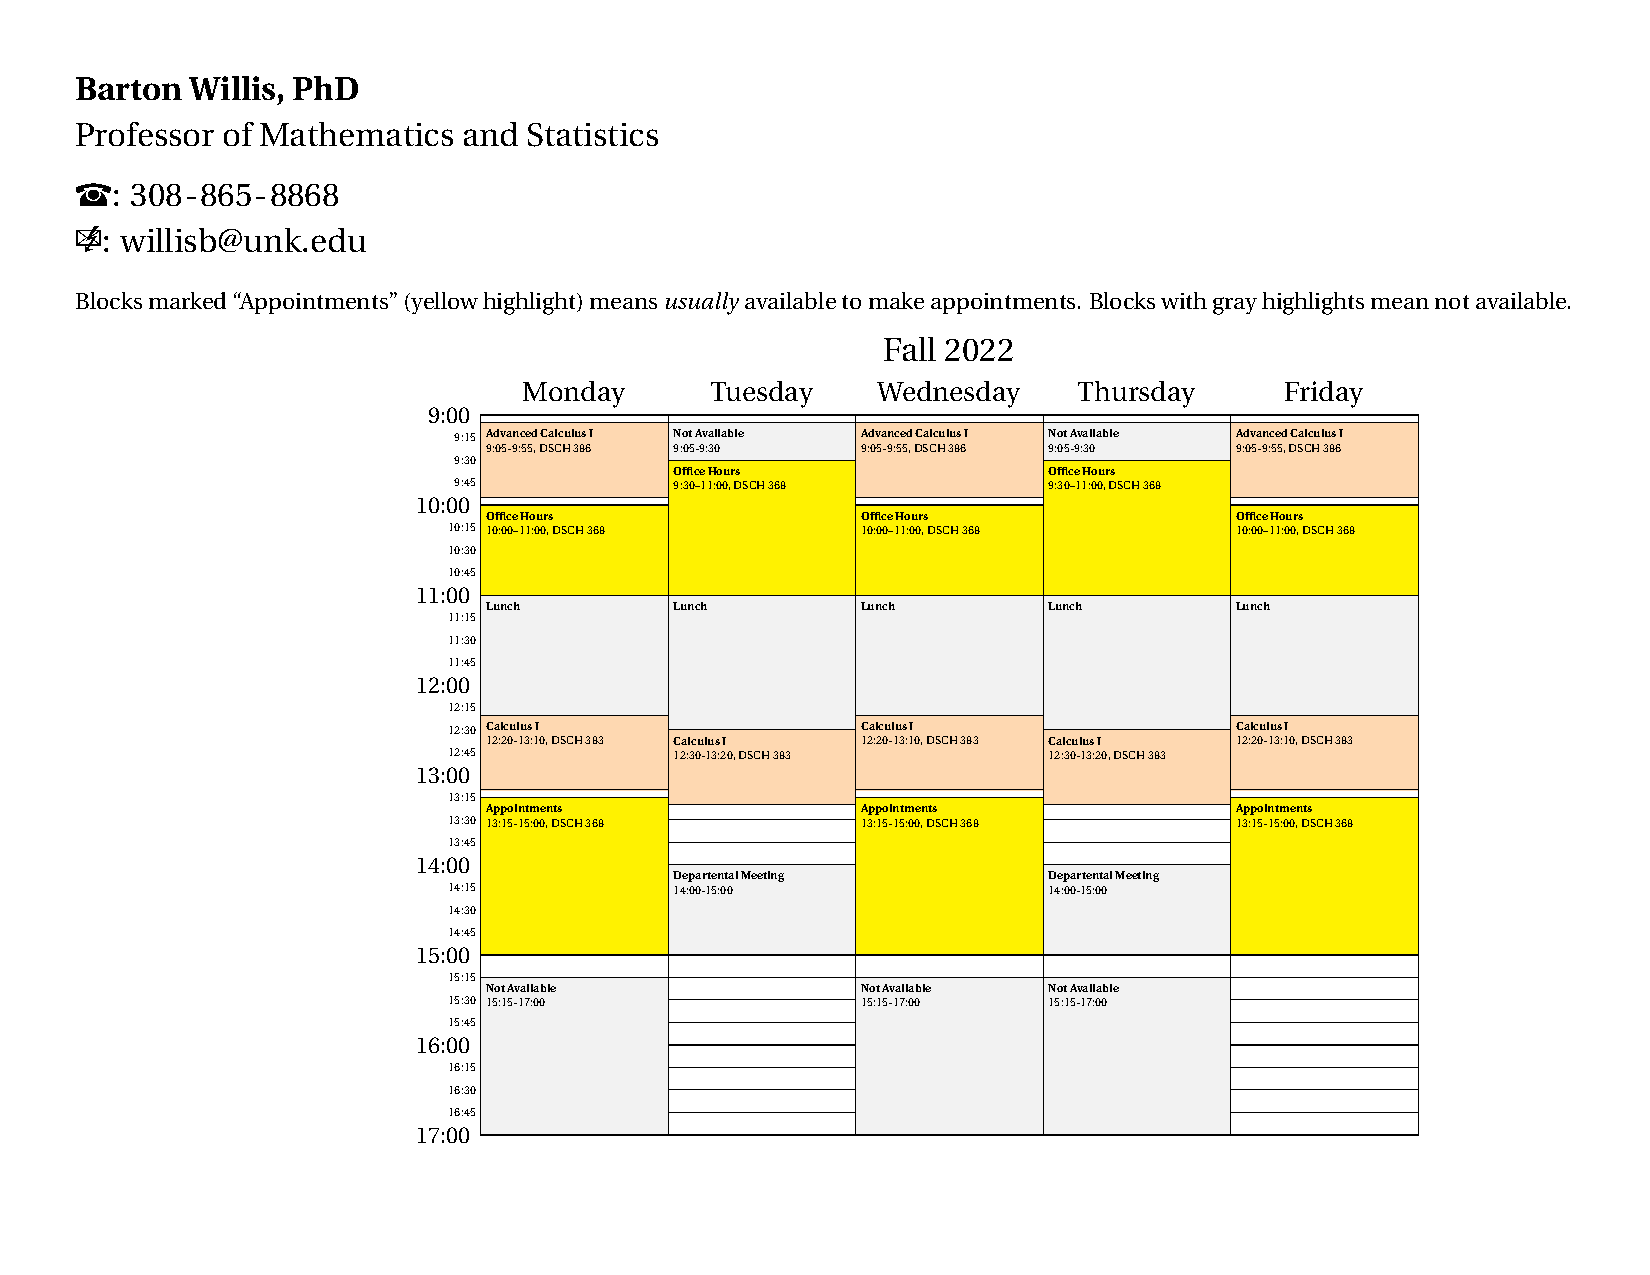
\includepdf[pages={1-},angle=90]{door_schedule.pdf}  
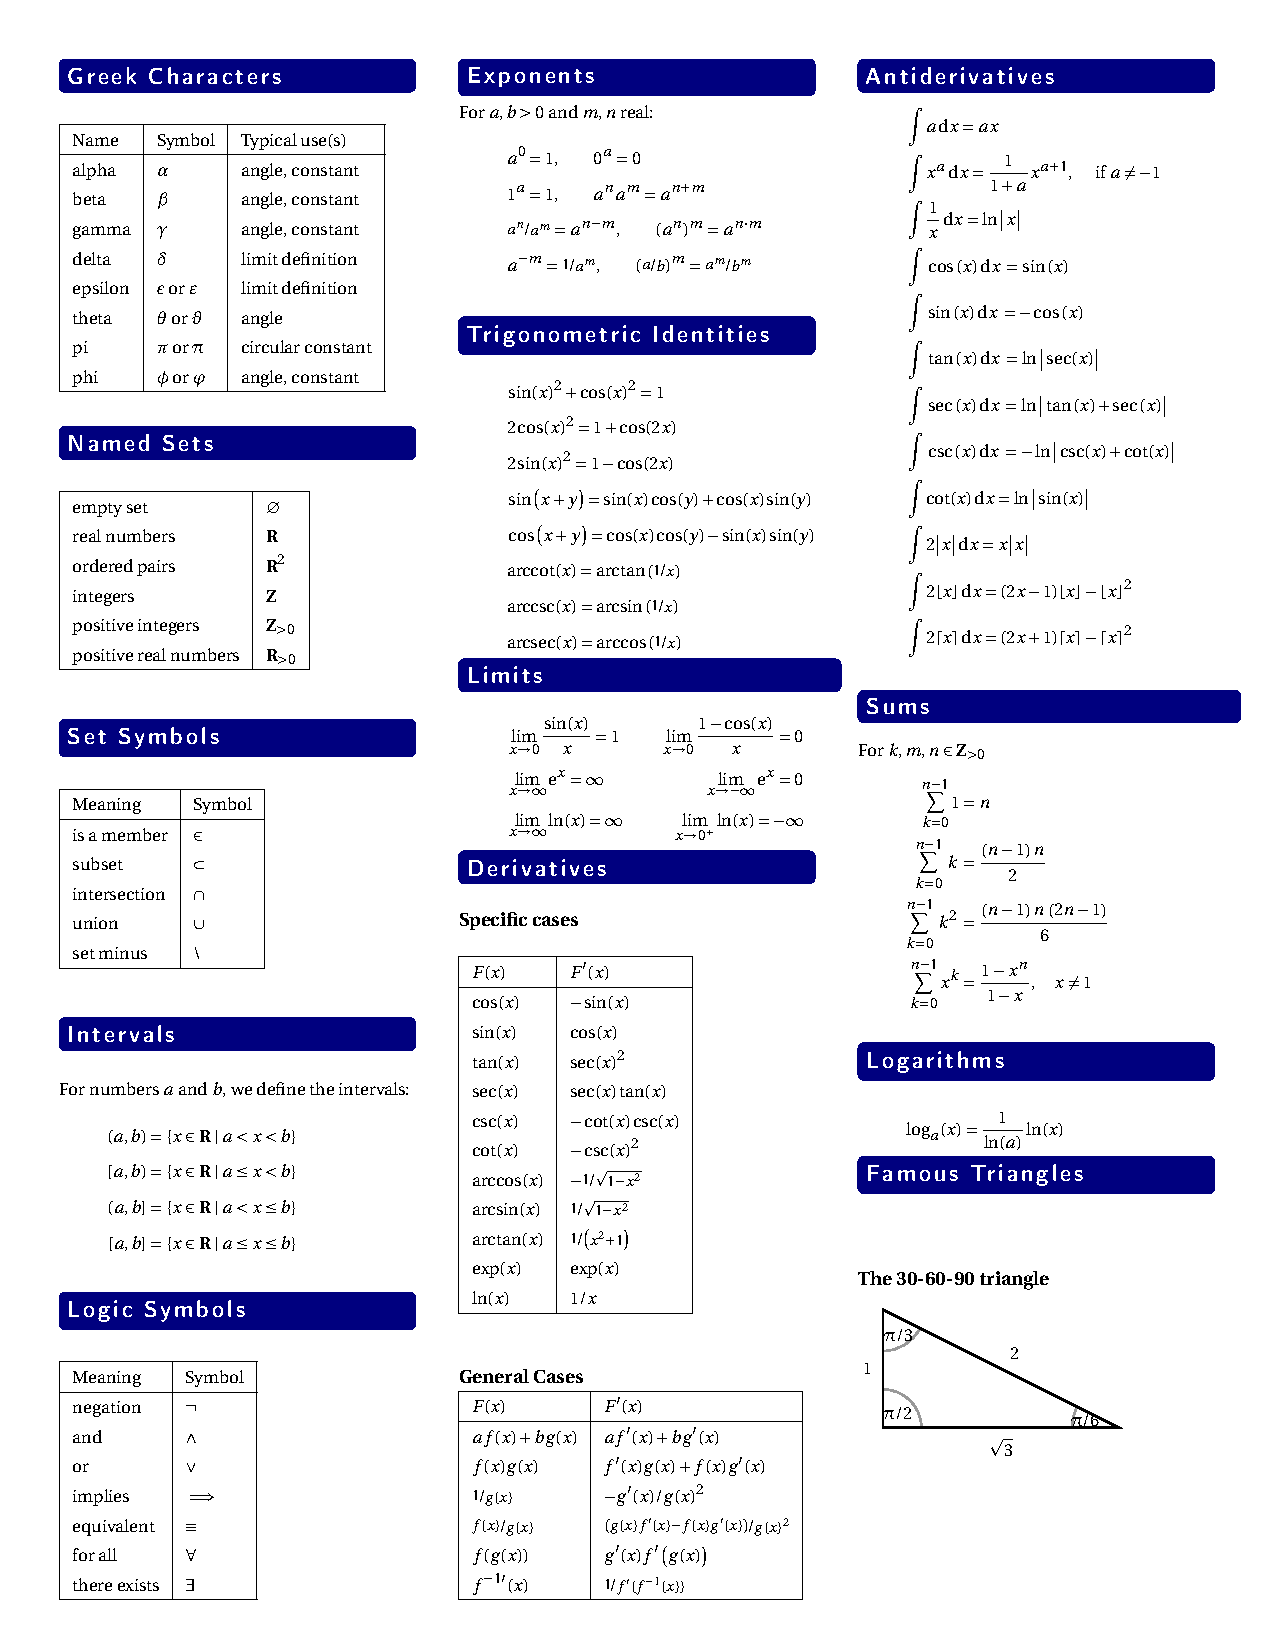
\includepdf[pages={1-},angle=90]{calculus-1-quick-reference.pdf} 

\end{document}


    

